\documentclass[tid,table]{texufpel} %use tid para doutorado e ti para mestrado



\usepackage{enumerate}
\usepackage[utf8]{inputenc} % acentuacao
\usepackage{graphicx} % para inserir figuras
\usepackage{url}

\hypersetup{
    hidelinks, % Remove coloração e caixas
    unicode=true,   %Permite acentuação no bookmark
    linktoc=all %Habilita link no nome e página do sumário
}

\usepackage{xcolor}
\usepackage{tabularx}
\usepackage{tablefootnote}

\usepackage{pdflscape}
\usepackage{afterpage}
\usepackage{capt-of}% or use the larger `caption` package

\usepackage[color=green!40]{todonotes}
\newcommand {\AY} {\todo[inline, color=green]} %comentarios Adenauer
\newcommand {\AP} {\todo[inline, color=yellow]} %Comentarios Ana

\unidade{Centro de Desenvolvimento Tecnológico}
\programa{Programa de Pós-Graduação em Computação}
\curso{Ciência da Computação}


\title{Avaliação de Estratégias de Segurança Adaptativa para a Internet das Coisas}


% VER ORIENTACAO DO LUCAS

\author{Almeida}{Ricardo Borges}
\advisor[Prof\textsuperscript{a}.~Dr\textsuperscript{a}.]{Pernas}{Ana Marilza}
\coadvisor[Prof.~Dr.]{Yamin}{Adenauer Corrêa}
\coadvisor[Sr.]{Donato}{Lucas Medeiros}

\keyword{Internet das Coisas}
\keyword{Segurança Adaptativa}
\keyword{Ciência de Contexto}

%Palavras-chave em EN_US
\keywordeng{Internet of Things}
\keywordeng{Adaptive Security}
\keywordeng{Context Awareness}
%\keywordeng{keyword-four}

\begin{document}

%\renewcommand{\advisorname}{Orientadora}           %descomente caso tenhas orientadora
\renewcommand{\coadvisorname}{Coorientadora}      %descomente caso tenhas coorientadora

\maketitle 

\sloppy

%\fichacatalografica


\begin{abstract}
Uma materialização da Computação Ubíqua que vem ganhando destaque é a Internet das Coisas (IoT), a qual consiste de um ecossistema que combina redes de sensores com e sem fio, computação em nuvem, dados analíticos, tecnologias interativas, bem como dispositivos inteligentes. A IoT atualmente inclui uma gama diversificada de dispositivos, serviços e redes para se tornar uma internet de qualquer coisa, em qualquer lugar, de qualquer forma e a qualquer momento. Com isso, os desafios de segurança e privacidade se potencializaram enquanto características necessárias e viabilizadoras para IoT. Promover a segurança com mecanismos pré-definidos e estáticos sobre este ambiente dinâmico e heterogêneo não se mostra mais uma abordagem oportuna. Por isso, são necessárias soluções para segurança auto-adaptativa. Tendo isto em vista, os objetivos deste trabalho consistem em: (i) sistematizar e apresentar os conceitos sobre segurança adaptativa para IoT, incluindo a sua relação com os estudos em ciência de contexto; (ii) realizar um mapeamento sistemático da literatura buscando identificar o estado da arte em segurança adaptativa para IoT; e (iii) desenvolver uma análise crítica sobre os trabalhos identificados em um esforço para elencar as lacunas existentes nesta área.
\end{abstract}


\begin{englishabstract}%
  {Assessment of Adaptive Security Strategies for the Internet of Things}
One of Ubiquitous Computing most prominent materializations is the Internet of Things (IoT), which consists of an ecosystem that combines wireless and wired sensor networks, cloud computing, analytical data, interactive technologies as well as intelligent devices. IoT currently includes a diverse range of devices, services and networks to become an internet of anything, anywhere, any way and anytime. As a result, the security and privacy challenges have become potentialized as a necessary and viable feature for IoT. Promoting security over this dynamic and heterogeneous environment with pre-defined and static security mechanisms is a challenging task. Therefore, solutions for self-adaptive security are required. The objectives of this work are: (i) systematize and present the concepts of adaptive security for IoT, including its relation with studies in context awareness; (ii) perform a systematic mapping of the literature striving to identify the state of the art in adaptive security for IoT; and (iii) develop a critical analysis of the work identified in an effort to fill the gaps in this area.
\end{englishabstract}

%Lista de Figuras
\listoffigures

%Lista de Tabelas
\listoftables

%lista de abreviaturas e siglas
\begin{listofabbrv}{SPMDRT}
	
       
	\item[UbiComp] \textit{Ubiquitous Computing}
	\item[IoT] \textit{Internet of Things}
	\item[MQTT] \textit{Message Queuing Telemetry Transport}
	\item[EP] \textit{Event Processing}
	\item[CEP] \textit{Complex Event Processing}
	\item[ESP] \textit{Event Streaming Processing}
        
\end{listofabbrv}

%Sumario
\tableofcontents

%\listoftodos
%%%%%%%%%%%%%%%%%%%%%%%%%%%%%%%%%%%%%%%%%%%%%%%%%%%%%%%%%%%%%%%%%%%%%%%
\chapter{Introdução}

A computação ubiqua (Ubiquitous Computing - UbiComp) apresenta como um de seus objetivos  disponibilizar a computação de forma integrada ao mundo físico tornando esta imperceptível aos usuários os quais não necessitam interagir com o gerenciamento da infraestrutura, fazendo apenas o uso da tecnologia sem quaisquer preocupações. Uma tecnologia emergente que tem se mostrado ser de certa forma uma materialização da computação ubiqua é a Internet das Coisas (Internt of Things - IOT), esta nova tecnologia consiste da integração de redes com dispositivos sem fio, computação em nuvem, dados analíticos, tecnologias interativas, bem como dispositivos inteligentes \cite{weiser1999computer}. 

A internet das coisas tem o potencial de mudar tudo ao nosso redor, adicionando "inteligência" aos mais variados itens do nosso dia a dia, visando  fornecer a seus usuários algum tipo de serviço. Para atingir este objetivo a ideia básica abordada pela IoT consiste em fazer com que diferentes tipos de dispositivos se comuniquem, interagindo e cooperando entre si para que deste modo, estes possam atingir um objetivo comum, como o fornecimento de um serviço qualquer para um usuário final. As áreas de aplicação para a IoT são das mais diversas possíveis, desde o uso em cidades grandes aplicando sensores visando fornecer diferentes tipos de serviços a sua população como por exemplo informações sobre o tráfego e eventos públicos, como o uso na agricultura com o intuito de executar um monitoramento preciso de  informações sobre as plantas e solo \cite{gonccalves2017research}.

Porém para que a internet das coisas se torne efetivamente uma realidade, presente nos mais diferentes lugares e servindo a todos os tipos de usuários e não apenas a especialistas, a comunidade científica precisa encontrar soluções para superar alguns desafios presentes nesse novo paradigma. Heterogeneidade da rede, como a IoT visa que os mais variados dispositivos podem estar presentes em uma rede trabalhando junto, a desafios presentes na forma como os dados gerados por esses diferentes dispositivos devem ser tratados tendo em vista que como estes são dispositivos potencialmente com hardwares e recursos totalmente diferentes as informações geradas por estes são muito discrepantes não havendo nenhum padrão no formato dos dados seguido atualmente \cite{agrawal2013survey}. O grande volume de dados gerados por estas redes de dispositivos, já que potencialmente as redes poderão conter dezenas de milhares de dispositivos interconectados se comunicando constantemente e gerando dados continuamente, onde estes, na maior parte dos casos precisam ser processados e analisados. A configuração desses dispositivos a qual deve ser feita de forma simplificada já que usuários finais sem conhecimentos técnicos precisam ser capazes de adicionar e remover dispositivos e recursos de uma rede sempre que estes desejarem. A segurança aplicada sobre estas redes, tendo em vista que soluções comuns de segurança não podem ser aplicadas sobre estas redes,  devido a grande variedade de dispositivos presentes nestas redes, onde muitos destas "coisas" conectados podem potencialmente apresentar hardwares simples de baixo poder computacional que não tem capacidade para executar técnicas de criptográficas modernas \cite{agrawal2013survey}.


Algumas previsões nos mostram que o há um crescimento constante no número de dispositivos conectados, em 2020 serão mais de 50 bilhões de dispositivos conectados a internet, tais perspectivas nos mostram que a IoT é um futuro próximo o que enfatiza a necessidade do desenvolvimento de soluções que sejam capaz de resolver os problemas citados de forma eficiente \cite{xavier2016smart}.


O restante deste trabalho esta organizado da seguinte forma. O capítulo \ref{cap:Embasamento_Teorico} onde é apresentado o embasamento teórico necessário para a compreensão da discussão levantada sobre os trabalhos identificados no mapeamento sistemático elaborado. No capítulo \ref{cap:Estado_da_Arte} é apresentado a execução do mapeamento sistemático elaborado por este documento, ainda é apresentado uma discussão sobre os trabalhos de interesse identificados durante o mapeamento sistemático. Por fim no Capitulo \ref{cap:Consideracoes_Finais} é apresentado as considerações finais obtidas com o desenvolvimento deste trabalho.



\chapter{Embasamento Teórico}
\label{cap:Embasamento_Teorico}

Neste capítulo será apresentado ao leitor o embasamento teórico sobre internet das coisas (\textit{Internet of Things} - IoT) apresentando seus principais objetivos e desafios a serem superados, ainda neste capítulo será abordado o conceito de processamento de eventos(\textit{Event Processing} - EP) uma grande área de pesquisa científica, a qual pode ser subdividida em outras duas principais áreas: o processamento de fluxo de eventos(\textit{event stream processing} - ESP), que se caracteriza por ter a capacidade de executar operações contínuas como filtros, agregações, classificações e junções, sob fluxos de dados; e o processamento de eventos complexos (\textit{complex event processing} - CEP) o qual faz uso de padrões pré definidos, aplicando-os sobre sequências de eventos simples, para assim fazer a detecção de eventos compostos \cite{dayarathna2018recent}. Na figura \ref{fig:ConjuntoProcessamento} é ilustrada a relação associativa entre estas três tecnologias, onde o processamento de eventos pode ser visto como um conceito mais genérico o qual engloba ESP que por sua vez engloba o CEP.

Nas seções seguintes deste capítulo será apresentado ao leitor o embasamento teórico necessário, sobre internet das coisas e processamento de Eventos, para que assim este possa ter uma melhor compreensão dos trabalhos apresentados no capítulo \ref{cap:Estado_da_Arte}.


\begin{figure}[ht]
	\centering
	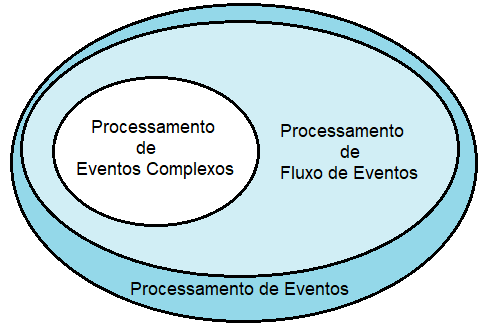
\includegraphics[width=.6\textwidth]{imagens/ConjuntoProcessamento.png}
	\caption{Conjunto de associação de processamento.}
	\label{fig:ConjuntoProcessamento}
\end{figure}


\section{Internet das Coisas}

A tecnologia computacional vem avançando consideravelmente nos últimos anos onde dispositivos cada vez menores com capacidade de se comunicar em rede com alto poder computacional estão se tornando cada vez mais comuns no dia dia. Esta popularização do uso desses dispositivos "inteligentes" tem sido chamada de internet das coisas, onde este novo paradigma computacional vem mudando a forma como as pessoas interagem com os objetos de seu cotidiano \cite{xavier2016smart}.

A internet das coisas tem o potencial de mudar tudo ao nosso redor, adicionando "inteligência" aos mais variados itens do nosso dia a dia, visando  fornecer a seus usuários algum tipo de serviço. Para atingir este objetivo a ideia básica abordada pela IoT consiste em fazer com que diferentes tipos de dispositivos se comuniquem, interagindo e cooperando entre si para que deste modo, estes possam atingir um objetivo comum, como o fornecimento de um serviço qualquer para um usuário final. As áreas de aplicação para a IoT são das mais diversas possíveis, desde o uso em cidades grandes aplicando sensores visando fornecer diferentes tipos de serviços a sua população como por exemplo informações sobre o tráfego e eventos públicos, como o uso na agricultura com o intuito de executar um monitoramento preciso de  informações sobre as plantas e solo \cite{gonccalves2017research}.

Porém para que a internet das coisas se torne efetivamente uma realidade, presente nos mais diferentes lugares e servindo a todos os tipos de usuários e não apenas a especialistas, a comunidade científica precisa encontrar soluções para superar alguns desafios presentes nesse novo paradigma. Heterogeneidade da rede, como a IoT visa que os mais variados dispositivos podem estar presentes em uma rede trabalhando junto, a desafios presentes na forma como os dados gerados por esses diferentes dispositivos devem ser tratados tendo em vista que como estes são dispositivos potencialmente com hardwares e recursos totalmente diferentes as informações geradas por estes são muito discrepantes não havendo nenhum padrão no formato dos dados seguido atualmente \cite{agrawal2013survey}. O grande volume de dados gerados por estas redes de dispositivos, já que potencialmente as redes conterão dezenas de milhares de dispositivos interconectados se comunicando constantemente e gerando dados continuamente, onde estes, na maior parte dos casos precisam ser processados e analisados. A configuração desses dispositivos a qual deve ser feita de forma simplificada já que usuários finais sem conhecimentos técnicos precisam ser capazes de adicionar e remover dispositivos e recursos de uma rede sempre que estes desejarem. A segurança aplicada sobre estas redes, tendo em vista que soluções comuns de segurança não podem ser aplicadas sobre estas redes,  devido a grande variedade de dispositivos presentes nestas redes, onde muitos destas "coisas" conectados podem potencialmente apresentar hardwares simples de baixo poder computacional que não tem capacidade para executar técnicas de criptográficas modernas \cite{agrawal2013survey}.


Algumas previsões nos mostram que o há um crescimento constante no número de dispositivos conectados, em 2020 serão mais de 50 bilhões de dispositivos conectados a internet, tais dados nos mostram que a IoT é um futuro próximo o que enfatiza a necessidade do desenvolvimento de soluções que sejam capaz de resolver os problemas citados de forma eficiente \cite{xavier2016smart}.

\section{Definição de Evento}
A definição de evento considerada neste documento é definida como a ocorrência de uma determinada ação dentro de um ambiente, que geralmente envolve uma tentativa de mudança de estado do sistema. Esta mudança inclui, normalmente, a noção de tempo, localidade e detalhes pertencentes ao evento ou a anomalia que desencadeou determinado evento que visam ajudar a compreender as causas ou efeitos desencadeadores do evento \cite{fitzgerald2010common}.
Um evento também pode ser separado em campos que descrevem suas propriedades, como por exemplo um evento em uma rede IoT pode incluir quatro atributos: eventID, eventName, eventTime e recordTime. EventID e eventName são normalmente definidos como registros básicos e são armazenados no data center, eventTime e recordTime expressam o conceito de tempo no evento descrevendo sua hora de ocorrência e de captura respectivamente \cite{minbo2013information}. 

Tais eventos podem ser aplicados em diversos sistemas para se atingir determinados fins, como por exemplo o uso em ferramentas de monitoramento onde estes eventos são utilizados para representar mudanças em situações \cite{etzion2011event}. Estes sistemas monitorados podem ser representados por conjuntos de sensores, onde por exemplo, em aplicações na agricultura de precisão são usados para o monitoramento da umidade e acidez do solo, de forma que tais valores emitidos por estes sensores podem ser vistos como mudanças de estado do ambiente, como uma mudança brusca na acidez do solo ou em sua umidade, as quais podem ser representadas como uma mudança de situação de interesse \cite{garcia2011wireless}.

\section{Definição de Processamento de Eventos}
O processamento de eventos pode ser visto como um paradigma onde fluxos de eventos são analisados continuamente com o objetivo de extrair informações úteis de alto nível destes dados analisados. Existem diversas áreas que possuem características com potencial de serem exploradas pelo processamento de eventos, dentre estas pode-se citar os setores da saúde com o monitoramento do status da saúde dos paciente onde os diversos eventos precisam ser processados e analisados \cite{weiner2008health}; o setor da agricultura de precisão o qual emprega diversos sensores para o monitoramento de plantas, gerando grandes fluxos de eventos que necessitam ser processados \cite{garcia2011wireless} e o setor de energia fazendo uso de eventos para o monitoramento do consumo excessivo de energia visando atingir uma eficiência energética melhor \cite{vijayaraghavan2010automated}. 

Apesar do processamento de eventos ser aplicado para resolver problemas em áreas totalmente distintas, existem alguns requisitos exigidos por estes que são normalmente semelhantes, tais como a necessidade de processar em tempo de execução grandes volumes de dados. Um setor em constante  crescimento que tem gerado grandes interesses no processamento de eventos é a Internet das Coisas(\textit{Internet of Things} - IOT) onde processamento de eventos tem se aplicado visando solucionar problemas de tomadas de decisão a partir da análise de grandes volumes de dados gerados por estas redes, diversas ferramentas foram desenvolvidas para o processamento de eventos, visando auxiliar na análise desse grande volume de dados, dentre estas pode-se citar o Apache Storm\footnote{\url{https://storm.apache.org/}}, Apache Spark\footnote{\url{https://spark.apache.org/}} e Apache Flink\footnote{\url{https://flink.apache.org/}}.

\subsection{Definição de Processamento de Fluxo de Eventos}

Para uma melhor e simples compreensão do significado de processamento de fluxo de eventos pode-se separar esta classe em outras três subclasses menores:
%já separasses na seção anterior, na verdade ela é uma fusão de outros conceitos
\begin{enumerate}
	\item  \textbf{Evento -} pode-se definir evento neste contexto como qualquer ação que aconteça com um tempo claramente definido, onde o mesmo pode ser mensurado.  
	
	\item  \textbf{Fluxo -} é definido como um sequência constante e contínuo de eventos disparados por dispositivos, onde esta corrente de eventos são claramente ordenados pelo tempo.
	
	\item  \textbf{Processamento} - é basicamente a ação final de executar a análise sobre o conjunto de informações capturadas.
\end{enumerate}
Desta forma com a combinação destes três sub-termos pode-se dizer que o processamento de fluxo de eventos nada mais é que processo de analisar em tempo de execução fluxo de eventos disparados por dispositivos assim que estes são criados \cite{dayarathna2018recent}. 

O processamento de fluxo de dados trata da identificação de padrões ou relacionamentos significativos entre os fluxos de dados analisados a fim de detectar determinados padrões como a correlação de eventos, causalidade ou tempo.
Características presentes em sistemas com aplicabilidade de processamento de fluxo de eventos são a necessidade de analisar grandes fluxos de dados correlacionando estas informações, aplicando filtros em tempo de execução e dando uma resposta de forma imediata, \cite{appel2013event}.


%talvez aqui colocar o processamento distribuído de eventos, que será teu foco na revisao sistematica do próximo capitulo

\subsection{Definição de Processamento de Eventos Complexos}
O processamento de eventos complexos é uma paradigma da computação onde este é aplicada para o processamento e análise de conjunto de fluxos de informações em sistemas baseados em eventos, visando analisar a interação destes eventos entre si, sistemas que empregam esta tecnologia normalmente apresentam as seguintes características: a necessidade de se verificar e informar a ocorrência de uma ação composta, isto é, a necessidade de identificar que dado a ocorrência de uma ação A e B em um determinado intervalo de tempo, o sistema deve ser capaz de informar que tais ações em conjunto formam uma nova ação C, a qual tem um valor semântico distinto se comparado com A e B individualmente. Uma área com grande aplicabilidade para o processamento de eventos complexos que tem se destacado nos últimos anos é a Internet das Coisas que apresentam grandes fluxos de dados de fontes heterogêneas e que normalmente necessitam ser analisados em tempo de execução \cite{jun2014design}. 

Assim para definirmos o conceito de processamento de eventos complexos tomado no desenvolvimento deste documento, será executado uma separação deste termo mais complexo em outros dois sub-conceitos menores que o compõe com o objetivo de facilitar a sua compreensão, Processamento e eventos complexos onde pode-se definir processamento como o ato final de analisar as informações já coletadas pelo sistema e eventos complexos como um forma evento nova mais abstrata de alto nível inferida a partir de eventos simples. Mais especificamente pode-se definir um evento complexo como sendo a combinação de dois ou mais eventos simples com o objetivo de criar um novo evento de mais alto nível, por exemplo \cite{dayarathna2018recent}, em um data center onde sensores monitoram o uso do disco rígido do sistema e o uso de rede, os eventos de alto uso do disco repentinamente disparam, após a análise destes eventos o sistema pode "decidir" disparar um novo evento "possível ataque Hacker" onde a partir deste novo evento os administradores podem decidir tomar alguma decisão  baseada neste novo evento como por exemplo desligar da rede do data center \cite{wu2006high}. 

Assim quando combinamos esses dois sub-conceitos citados, tem-se que o processamento de eventos complexos é o ato de analisar conjuntos de fluxos de eventos simples, visando assim inferir a partir destes, um novo conjunto de eventos semanticamente distintos dos anteriores. Ou seja, pode-se dizer que a partir de uma analise combinatória de eventos simples o CEP é capaz de gerar um novo conjunto de informações, semanticamente de mais alto nível que as informações combinadas na análise.



%[Ana] Faltou falar em Processamento Distribuído de Eventos ou de Fluxo de Eventos 

%%%%%%%%%%%%%%%%%%%%%%%%%%%%%%%%%%%%%%%%%%%%%%%%%%%%%%%%%%%%%%%%%%%%%%% 
\chapter{Estado da Arte} 
\label{cap:Estado_da_Arte}

Neste capítulo é apresentado o estado da arte das pesquisas que tem como tema processamento de eventos e internet das coisas. Na seção seguinte é apresentado o protocolo seguido para a execução do mapeamento sistemático assim como todos os passos executados que levaram a escolha dos trabalhos de interesse. Por fim será apresentado uma discussão sobre as soluções abordadas nos trabalhos de interesse selecionados.    

\section{Mapeamento Sistemático da Literatura}

O mapeamento sistemático abordado neste capítulo é baseada na metodologia proposta por Petersen et al. (2008), onde seguindo a série de passos proposto, torna o estudo realizado, possível de ser replicado por outros pesquisadores \cite{petersen08}. A partir desta metodologia, pode ser citado cinco etapas das quais serão seguidas por este mapeamento:

\begin{enumerate}
	\item Definição das questões de pesquisa;
	\item Execução da pesquisa para identificação de estudos primários realizados;
	\item Triagem, inicial empregando critérios de inclusão e exclusão considerando o resumo dos artigos;
	\item Triagem final, considerando as seções de introdução, concepção do projeto e conclusão;
	\item Extração dos dados e mapeamento.
	

\end{enumerate}  

Para a consulta dos trabalhos relacionados primeiramente foi definido um conjunto de palavras como candidatas a palavras chave para a \textit{string} de busca, dentre estas pode-se citar: \textit{internet of things}, \textit{distributed} e \textit{complex event processing}. A Partir da definição destas como palavras chave, foi possível elaborar a \textit{string} de busca usada para executar as consultas sobre as bases da: ACM Digital Library, IEEE Explore, ScienceDirect, Springer, Web of Science e Scopus; e assim obter-se os trabalhos relacionados com o tema de pesquisa, as strings de consulta podem ser vistas na figura \ref{tab:stringBusca} incluindo em qual respectiva base estas foram executadas.



\begin{figure}[ht]
	\centering
	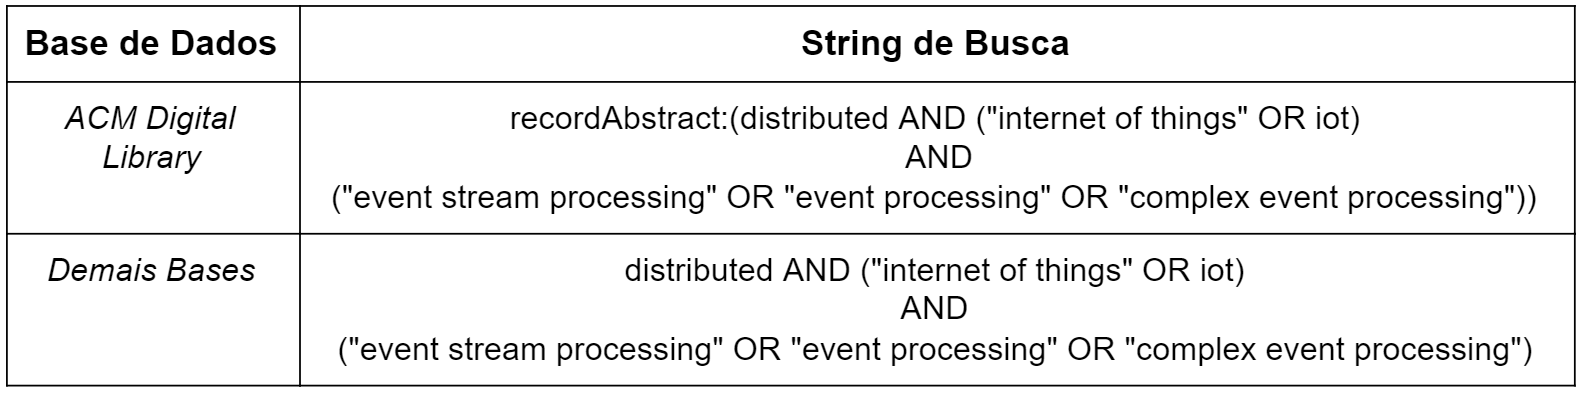
\includegraphics[width=1\textwidth]{imagens/tabela_string_busca.png}
	\caption{Strings de buscas usadas.}
	\label{tab:stringBusca}
\end{figure}

Após a execução desta consulta preliminar, que entende-se como a etapa de levantamento dos estudos primários relevantes, foram identificado 647 trabalhos de interesse onde este valor  compreende-se da soma dos resultados obtidos em todas as bases de consulta.

Todas as buscas foram realizadas sobre os metadados dos artigos(titulo, resumo e palavras chave), porem, como a base de dados Springer não oferecia suporte a este tipo de consulta, este problema foi contornado da seguinte forma: primeiramente foi feita a exportação do resultado preliminar da busca na base para o formato CSV(o único suportado) resultando em 472 artigos. Após isto fez-se uso da ferramenta CSV2Bib\footnote{\url{https://github.com/jacksonpradolima/csv2bib}} para converter o arquivo CSV para .bib com o intuito de importar o resultado, para a ferramenta Zotero\footnote{\url{https://www.zotero.org/}}, oque permitiu a execução da String de busca sobre os metadados dos 472 artigos encontrados preliminarmente, resultando em 6 documentos de interesse. A figura  \ref{fig:GrafBarraPubAno} apresenta um gráfico de barras contendo o número de artigos encontrados pela \textit{string} de busca em cada uma das bases, já a figura \ref{fig:GrafPizPubAno} apresenta o percentual de publicações que cada uma das bases contribuiu para o montante final.

\begin{figure}[ht]
	\centering
	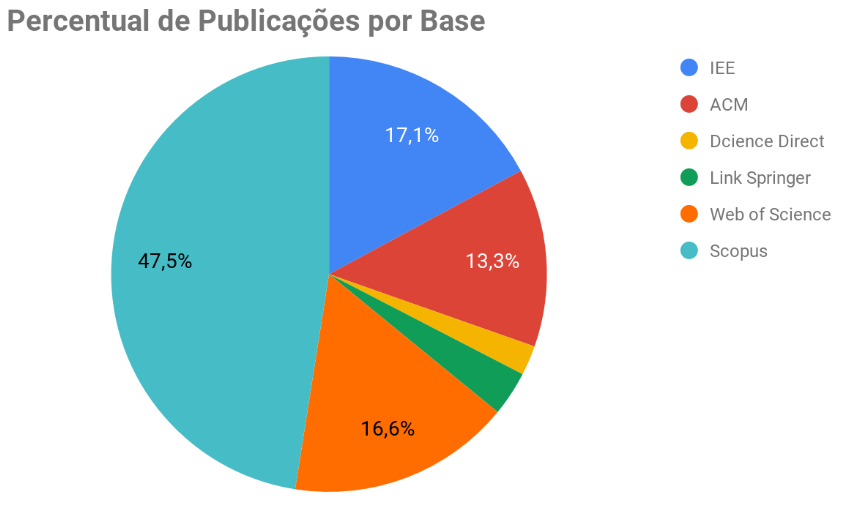
\includegraphics[width=.9\textwidth]{imagens/GrafPizPubAno.png}
	\caption{Percentual de publicações encontradas por base.}
	\label{fig:GrafPizPubAno}
\end{figure}

\begin{figure}[ht]
	\centering
	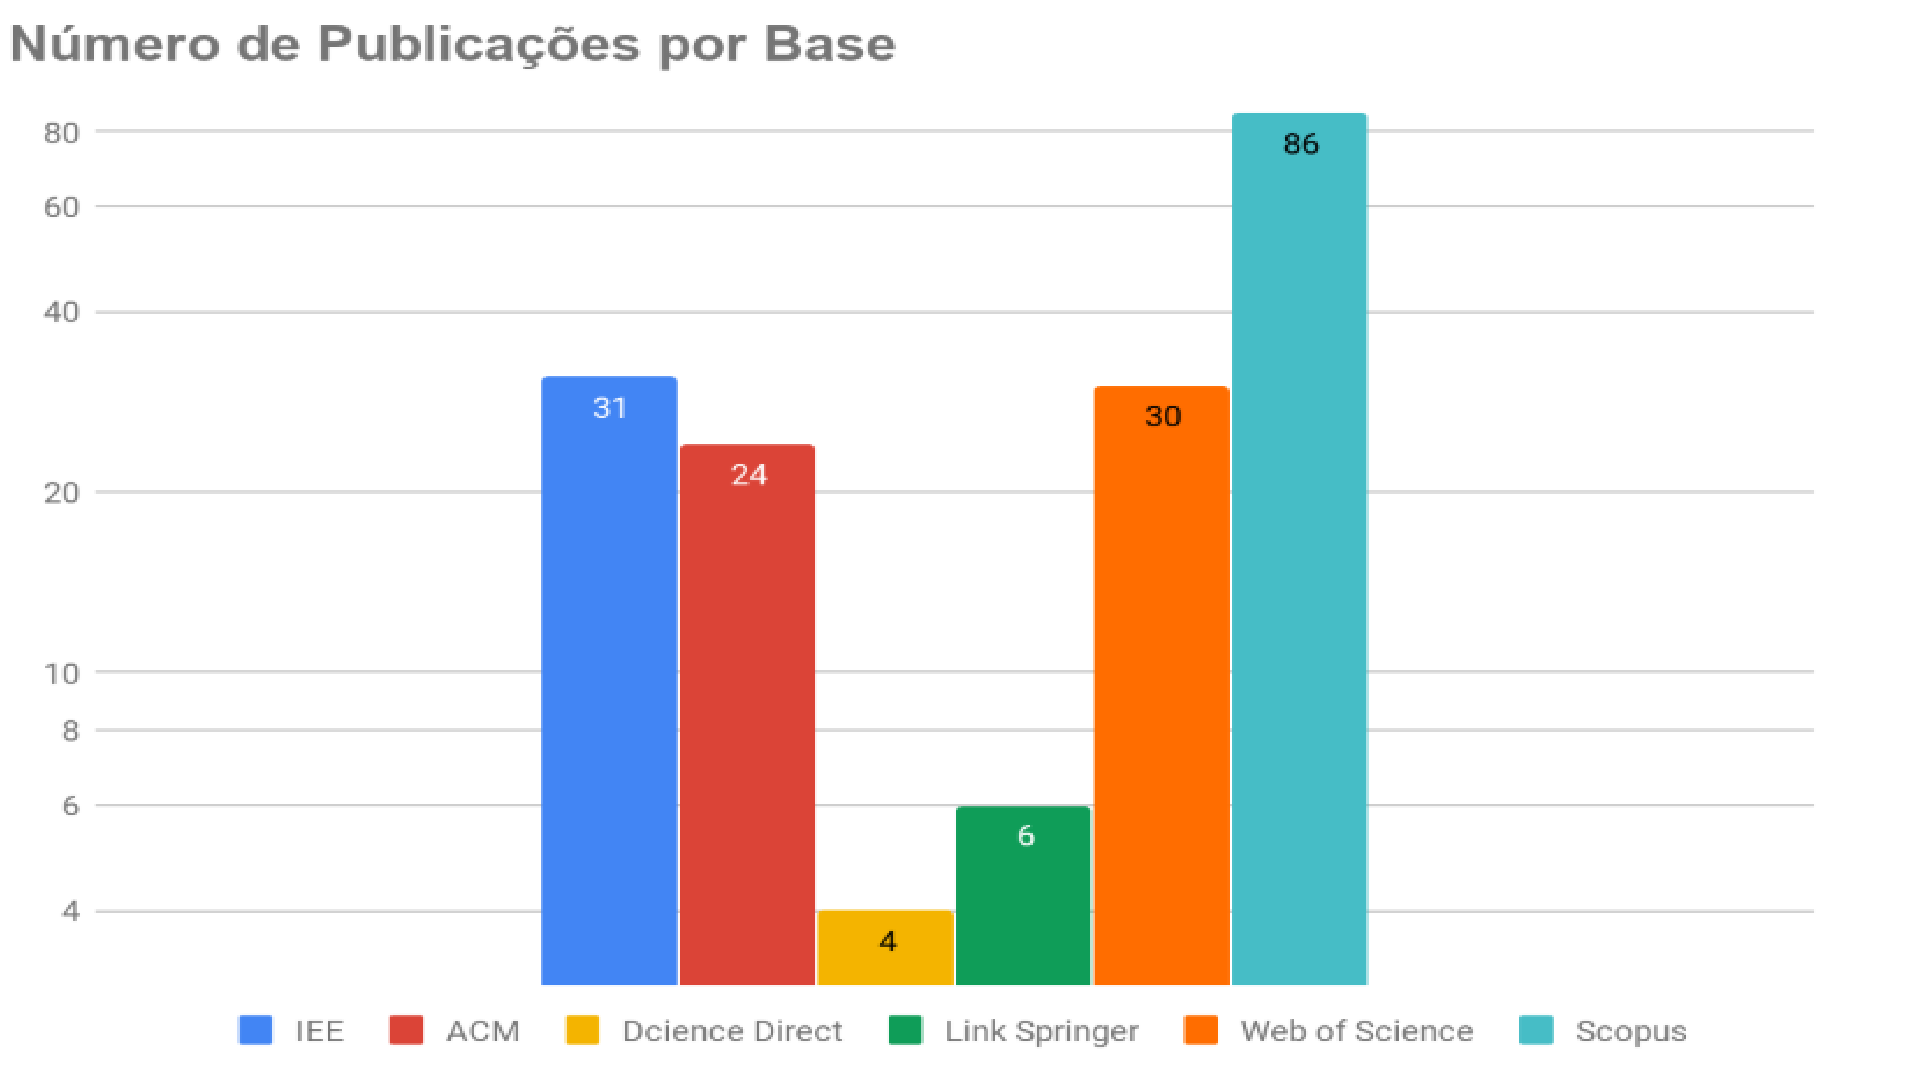
\includegraphics[width=.9\textwidth]{imagens/GrafBarraPubAno.png}
	\caption{Número de publicações encontradas por base.}
	\label{fig:GrafBarraPubAno}
\end{figure}


O gráfico \ref{fig:grafPublicaAno} apresenta o número de publicações de interesse encontradas e cada uma das bases. O eixo X apresenta o ano do qual os artigos foram publicados e o eixo Y apresenta o número total de publicações em relação ao ano. Para a representação do gráfico foram removidas todas as publicações duplicadas. Podem-se perceber pela figura \ref{fig:grafPublicaAno} que a partir do ano de 2015 há um considerável aumento no número de publicações, e ainda um grande pico no ano de 2017, demonstrando assim pontos de interesse neste período de publicações.

\begin{figure}[ht]
	\centering
	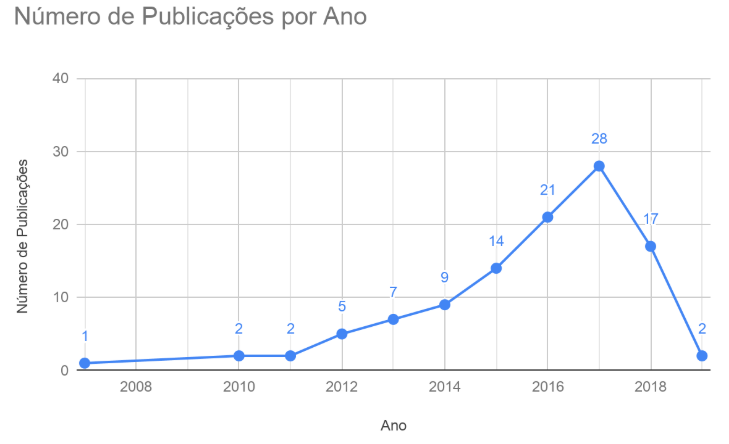
\includegraphics[width=.9\textwidth]{imagens/grafPublicaAno.png}
	\caption{Quantidade de publicações de interesse por ano.}
	\label{fig:grafPublicaAno}
\end{figure}

\subsection{Critérios de Inclusão e Exclusão}
Após a seleção inicial realizada sobre as bases de dados, executou-se a triagem inicial sobre o resumo dos artigos, aplicando os seguintes critérios de inclusão e exclusão conforme a ordem apresentada abaixo: 
\begin{itemize}
	\item (E) Foi publicado antes de 2015;
	\item (E) Não é um artigo \textit{full paper};
	\item (E) Não esta em Inglês ou Português;
	\item (E) Indisponibilidade de acesso ao artigo completo;
	\item (E) Artigos que não apresentam avaliação da proposta;
	\item (I) Explora conceitos de segurança;
	\item (I) Explora conceitos de Computação Ubíqua;
	\item (E) O artigo não possui nenhum dos critérios de inclusão.
\end{itemize}
	
Para auxiliar na aplicação dos critérios de inclusão e exclusão foi feita a importação dos resultados preliminares das buscas na ferramenta Start\footnote{\url{http://lapes.dc.ufscar.br/tools/start_tool}},
para isso usou-se os arquivos .bib exportados pelas ferramentas das bases de busca, com exceção apenas da Spriger, onde usou-se o arquivo .bib exportado pelo Zootero, que foi gerado apos a execução da consulta sobre os metadados, aplicada sobre o resultado preliminar da base.

Os critérios de exclusão foram aplicados seguindo a seguinte ordem e etapas:

\begin{itemize}
	\item  \textbf{Remoção de Trabalhos Duplicados - } Muitos dos trabalhos retornados pela \textit{string} de busca estavam indexados em ambas as bases de consulta, tornando necessário a execução de uma etapa de remoção dos mesmos, resultando em 74 trabalhos duplicados removidos.
	
	\item  \textbf{Filtro por Data - } O intervalo de interesse para a aplicação do filtro foi adotado com base no número de publicações por ano. Após o levantamento dos trabalhos de interesse, identificou-se o ano de 2015 como sendo o ano em que o número de publicações aumenta considerável mente, continuando a ascender até o pico máximo no ano de 2017, como pode ser visto na figura \ref{fig:grafPublicaAno}. Assim optou-se por eliminar todas as publicações que fossem anteriores ao ano de 2015 eliminando desta forma 26 artigos.	
	
	\item  \textbf{Artigos Full Paper - } Com o intuito de remover artigos que apresentassem apenas resumos superficiais sobre os trabalhos, ou que não tivesse apelo científico, optou-se por remover artigos que não sejam Full Paper (livro ou capítulo de livro, introdução de anais, entre outros), sendo removidos 9 trabalhos.
	
	\item  \textbf{Filtro por Idioma - } Como as pesquisas foram realizadas sobre varias bases de dados onde muitas destas indexam trabalhos em vários idiomas, optou-se por usar um filtro por idioma para remover qualquer trabalho que não esteja em Português ou Inglês(idiomas de total domínio do autor) removendo desta forma 1 artigo.
	
	\item  \textbf{Indisponibilidade do Artigo completo - } Dado que alguns dos estudos de interesse selecionados apresentaram apenas seus resumos e introdução disponíveis não oferecendo a opção de obter-se o trabalho completo, optou-se por remover estes do pesquisa, sendo excluído 3 trabalhos.
	
	\item  \textbf{Avaliação da Proposta - } Foram removidos todos os artigos que não executaram algum tipo de teste ou estudo de caso das soluções propostas por seus trabalhos, excluindo assim 17 artigos.
	
	\item  \textbf{Sem Nenhum Critério de Inclusão - } Todos trabalhos que não  se enquadraram em nenhum dos critério de inclusão foram removidos, excluindo desta forma 28 trabalhos da pesquisa.	

\end{itemize}


Após execução da triagem inicial dos trabalhos, aplicando os critérios de inclusão e exclusão sobre o resumo dos artigos, selecionou-se 24 documentos de interesse, o fluxo da aplicação dos critérios de exclusão pode ser visto na figura \ref{fig:grafFluxoTriagemInicial} assim como o número total de trabalhos removidos por cada um dos critérios de aplicação. 

A execução da 4º etapa do mapeamento, que consiste da triagem final dos trabalhos de interesse, selecionou dez dos 24 artigos para analise completa de seu conteúdo e da extração das informações destes. O critério considerado para a seleção dos dez trabalhos foi se estes exploravam conceitos de segurança da informação ou ainda se estes apresentavam o uso de conceitos de Computação Ubíqua. 


\begin{landscape}
\begin{figure}[ht]
	\centering
	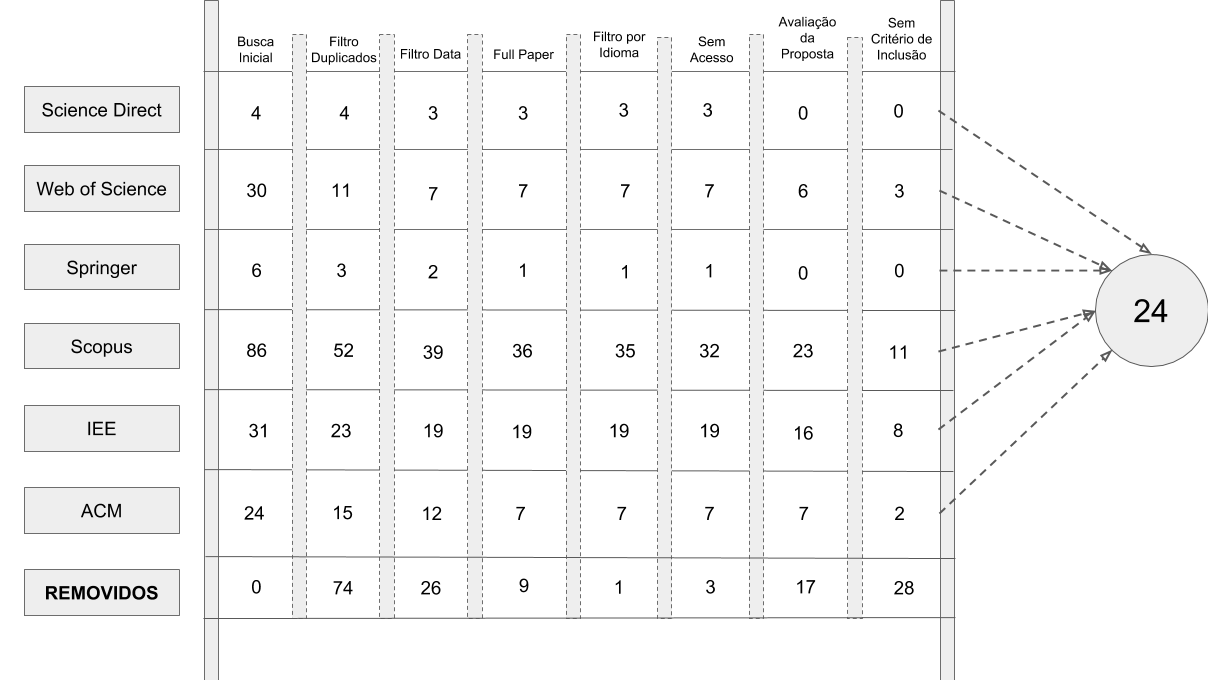
\includegraphics[width=1.7\textwidth]{imagens/FluxoTriagemInicial.png}
	\caption{Fluxo de triagem dos artigos.}
	\label{fig:grafFluxoTriagemInicial}
\end{figure}
\end{landscape}


\section{Trabalhos Relacionados}
Com a execução do mapeamento sistemático da literatura
foram selecionados dez trabalhos de interesse, os quais serão apresentados nas subseções a seguir, onde serão abordados os seguintes tópicos de interesse: motivação e justificativa do trabalho, solução apresentada, avaliação e Resultados da Proposta.


%%%%%%%%%%%%%%%%%%%%%%%%%%%%%%%%%%%%%%%%%%%%%%%%%%%%%%%%%%%%%%%%
\subsection{Towards a Generalized Approach for Deep Neural Network based Event Processing for the Internet of Multimedia Things}

\begin{itemize}
	\item \textbf{Motivação e Justificativa do Trabalho:} O uso de dispositivos IoT multimídia tem aumentado consideravelmente (uso de câmeras para monitorar o trafego de uma cidade por exemplo). Desta forma os tipos dos eventos criados na IoT estão também mudando, onde estes eventos multimédia geram dados não estruturados, gerando uma procura crescente na utilização eficiente do processamento de fluxos de eventos multimídia. No entanto, os mecanismos de processamento de eventos atuais têm suporte limitado ou inexistente para tipos de evento não estruturados \cite{art1aslam2018towards}.
	
	\item \textbf{Solução Apresentada:} É proposto um sistema genérico para manipular eventos da Internet das Coisas Multimídia (IoMT) como um tipo de evento nativo em ferramentas de processamento de eventos com alta eficiência. O sistema proposto estende as linguagens de processamento de eventos com a introdução de operadores para análise multimídia de eventos não estruturados (eventos multimídia). A ferramenta proposta faz uso de um combinador de eventos baseado em redes neurais convolucionais profundas para executar o processamento de eventos de imagem e assim extrair recursos destas \cite{art1aslam2018towards}.
	
	\item \textbf{Avaliação e Resultados da Proposta:} O sistema desenvolvido foi otimizado, com o uso de uma abordagem de seleção de classificadores baseado em restrições de assinatura. Os resultados obtidos pelos autores mostram que a ferramenta atinge uma taxa de transferência média de 110 quadros/segundo com uma precisão aproximada de 66,34\% em eventos do mundo real de várias aplicações de cidades inteligentes. Por fim foi apresentado um teste de desempenho com o aumento  gradativo do número de classes por classificador, onde os resultados obtidos mostram uma taxa de transferência estável para um classificador de uma classe, porem com o aumento do número destas classes a taxa de transferência cai continuamente \cite{art1aslam2018towards}.  
	
\end{itemize}


\subsection{A Web-based Approach using Reactive Programming for Complex Event Processing in Internet of Things Applications}

\begin{itemize}
	\item \textbf{Motivação e Justificativa do Trabalho:} Nos últimos anos a Internet das coisas (IoT) tem crescido substancialmente, aumentando progressivamente o número de dispositivos conectados a rede, estima-se que em poucos anos cada um dos objetos de uso comum irá conter sensores para coletar e/ou fornecer algum tipo informação ou serviço para seus usuários, se conectando na Internet e gerando cada vez mais uma enorme quantidade de dados para serem trafegados pela rede. Esse crescente aumento no número de dispositivos e consequentemente a grande expansão no volume de dados, gera a necessidade que seja desenvolvida uma abordagem simples para que se possa lidar com esta nova grande avalanche de dados \cite{art2zimmerle2018web}.
	
	\item \textbf{Solução Apresentada:}  É proposto pelos autores a combinação de duas abordagens distintas para solucionar o problema citado por estes da nova grande avalanche de dados gerados pelas redes IoT: o CEP(\textit{Complex Event Processing}) e WoT (\textit{Web of Things}) com o uso de Ferramentas gráficas que exploram programação de fluxo (Mashups) o que irá permitir o uso de operadores CEP em eventos de alto niveis visualmente criados na plataforma WoT.
	Para o desenvolvimento dos operadores CEP utilizou-se Programação Reativa, os quais foram fornecidos como uma extensão da plataforma WoT Node-RED\footnote{\url{https://nodered.org/}}, onde foram implementados três dos programas Coral8 amplamente referenciados para sistemas CEP, gerando a primeira extensão do CEP para a plataforma Node-RED, esta sendo uma ferramenta de programação construída em cima do Node.js, como protocolo de comunicação da troca de mensagens, os autores optaram por usar o MQTT\footnote{\url{https://mqtt.org/}}(\textit{Message Queuing Telemetry Transport}) \cite{art2zimmerle2018web}. 	
	
	\item \textbf{Avaliação e Resultados da Proposta:} Para a avaliação da proposta do trabalho, um cenário de caso de uso é apresentado onde para este fim usou-se o simulador node-red-node-pi-sense-hatsimulator, desenvolvido pela equipe Node-RED que tem como objetivo reproduzir uma placa real Raspberry PI a qual incorpora alguns sensores e atuadores como LEDs, temperatura, pressão barométrica e sensores de umidade, entre outros, os quais foram usados para a simulação dos CEP da proposta. Com o desenvolvimento deste trabalho os autores citaram duas como as principais contribuições da pesquisa: (1) uma abordagem visual para construir consultas CEP para aplicativos de Internet e (2) o uso de Programação Reativa para detectar e acionar o CEP \cite{art2zimmerle2018web}.
	
\end{itemize}


\subsection{Semantic IoT Middleware-enabled Mobile Complex Event Processing for Integrated Pest Management}

\begin{itemize}
	\item \textbf{Motivação e Justificativa do Trabalho:} Existem diversos desafios na agricultura moderna que são tipicamente encontrados no domínio dos Sistemas Ciber-Físicos (CPSs), dentre estes pode-se citar: conhecimento e deficiência de infraestrutura, informações incompletas, fontes limitadas de informação, perturbações externas (clima), autoridade de controle limitada (fertilizantes não podem fazer uma planta crescer arbitrariamente rápido). O gerenciamento agrícola moderno depende  de muitas metodologias diferentes de sensoriamento para fornecer informações precisas sobre a cultura, o clima e as condições ambientais. Graças a miniaturização, da grande evolução e da difusão de sensores e recursos computacionais de baixo custo, tornou-se possível o desenvolvimento de dispositivos que produzem dados e que interagem entre sí, produzindo assim uma rede de "coisas", gerando dados, processos e serviços interconectados. Desta forma os CPSs estão transformando a indústria agrícola \cite{art3nocera2017semantic}.
	
	\item \textbf{Solução Apresentada:} O trabalho propõe uma infraestrutura inteligente projetada para processar fontes de dados heterogêneas, como dados de sensores, dados meteorológicos e conhecimento agrícola coletado em uma ontologia, possibilitando uma comunicação mais suave e homogênea entre os dispositivos de uma infraestrutura dinâmica, configurável e extensível. A solução desenvolvida é baseada em processamento de eventos complexos (CEP) com o uso da ferramenta Esper\footnote{\url{http://www.espertech.com/}}, onde um modulo é executado parcialmente em dispositivos móveis através da introdução do DeviceHive, um \textit{middleware} da Internet das Coisas, ainda fez-se uso de uma linguagem de programação com suporte a mecanismos de reflexão, os quais servem como uma interface entre os componentes da IoT e o conhecimento ontológico. Para o sistema de comunicação entre o servidor e os dispositivos moveis é usado um \textit{middleware} de publicação/assinatura composto por um DSB (\textit{Distributed Service Bus}), um serviço do \textit{Google Cloud Messaging} e um serviço da Web de assinatura. Segundo os autores a solução visa tornar-se um instrumento utilizado para conscientizar sobre o uso dos tratamentos agrícolas, onde o agricultor pode (i) ter acesso a todas as informações relacionadas ao domínio de interesse no momento necessário, (ii) criar um plano de defesa personalizado, (iii) receber alertas de mudanças nas condições climáticas e (iv) receber notificações e recomendações sobre seus planos de tratamento \cite{art3nocera2017semantic}.

	
	\item \textbf{Avaliação e Resultados da Proposta:} Para a validação da proposta desenvolvida foi apresentado uma instanciação de um cenário real, projetando também uma Ontologia OWL(\textit{Ontology Web Language}) que codifica o conhecimento sobre aspectos relacionados à prática de Manejo Integrado de Pragas. Os autores executaram um primeiro conjunto de experimentos para validar a abordagem de fornecer a ferramenta para uma empresa e testar componentes individuais. Por fim os autores citaram como principais contribuições do trabalho: (i) a possibilidade de usar o motor CEP em tempo de execução do sistema, o que permite o monitoramento orientado a eventos e notificações de atualização, e (ii) sistema de modelagem com ontologias compreensíveis homem-máquina, que garante uma reconfiguração mais fácil a ferramenta \cite{art3nocera2017semantic}. 
	
\end{itemize}

\subsection{Predictive Analytics for Complex IoT Data Streams}

\begin{itemize}
	\item \textbf{Motivação e Justificativa do Trabalho:} Os CEP são capazes de fornecer soluções escaláveis e distribuídas para lidar com fluxos de dados complexos em tempo real, no entanto, os CEPs  não possuem a capacidade de realizar predições assim como muitas das técnicas de aprendizado de máquina e análise estatística de dados. A grande parte dos aplicativos CEP disponíveis  na literatura destina-se apenas a fornecer soluções reativas ao correlacionar fluxos de dados usando regras predefinidas, não explorando dados históricos devido a sua memória limitada. Existem diversos casos em que a predição de um evento futuro é muito mais útil que apenas a detecção do mesmo, por exemplo, seria muito mais útil a previsão de um congestionamento em uma auto estrada do que sua detecção, já que com a predição deste evento, com alguma antecedência, torna-se possível notificar aos administradores de trafego, para que estes possam tomar as medidas preventivas de modo a evitar o congestionamento. Pode-se citar ainda diversos outros casos onde a predição de eventos futuros podem trazer diversos ganhos como a previsão de desastres naturais e doenças epidêmicas \cite{art4akbar2017predictive}. 
	
     \item \textbf{Solução Apresentada:} Neste trabalho foi proposto uma arquitetura pró-ativa capaz de explorar dados históricos usando técnicas de aprendizado de máquina em conjunto com processamento de eventos complexos, de forma a combinar o poder do processamento de dados em tempo real do CEP com a capacidade de predição de eventos das técnicas de ML. Foi apresentado um algoritmo de predição adaptativo chamado de AMWR (\textit{Adaptive Moving Window Regression}) para dados dinâmicos de IoT, capaz de realizar predições precisas quase que em tempo real, e ainda sendo capaz de trabalhar em conjunto com o CEP. Para a execução da proposta os autores fizeram uso das seguintes ferramentas: Node-RED para fornecer o Front-End da arquitetura, o Apache Kafka\footnote{\url{https://kafka.apache.org/}} como Broker de mensagens e por ultimo, a implementação foi elaborada em Python com o uso do módulo de aprendizagem de máquina scikit-learn \cite{art4akbar2017predictive}.  
     
     
     
	 \item \textbf{Avaliação e Resultados da Proposta:}
	 Para avaliação da proposta foi elaborado um caso de uso do mundo real onde dados de trafego de sistemas de transportes inteligentes foram usados para os testes, onde o algoritmo de predição foi capaz de atingir uma precisão de 96\%, demonstrando assim a sua viabilidade de uso, já que com predições corretas sobre o trafego, como as que foram apresentadas nos testes, permitem que os administradores do sistema gerenciem o tráfego de uma maneira melhor, tomando decisões para evitar situações indesejadas, como congestionamentos por exemplo.	 
	 Os autores do artigo citam como principais contribuições do trabalho:
	 a implementação de uma arquitetura genérica baseada em componentes de código aberto para combinar ML com CEP, a fim de prever eventos complexos para aplicativos proativos de IoT;
	 o desenvolvimento de um algoritmo de predição adaptativo para fluxos de dados dinâmicos de IoT que foi implementado em um caso de uso real do ITS atingindo uma precisão de até 96\%. Também foi proposto um novo método para encontrar tamanho ótimo para janela de treinamento, explorando componentes espectrais de dados de séries temporais;
	 A modelagem do erro introduzido pelo algoritmo de previsão usando uma distribuição paramétrica e a derivação em expressões para o erro global do sistema, à medida que o erro se propaga através do CEP \cite{art4akbar2017predictive}.
\end{itemize}


\subsection{DRESS: A Rule Engine on Spark for Event Stream Processing}

\begin{itemize}
	\item \textbf{Motivação e Justificativa do Trabalho:} Nos últimos anos o número de dispositivo conectados a rede vem aumentando, com esse crescimento, a quantidade de fluxos de dados aumenta simultaneamente, gerando a necessidade de sistemas capazes de reagir automaticamente a determinados eventos desencadeados por fluxos de dados. Tais sistemas se baseiam em um conjunto de regras pre definidas, onde através da análise dos fluxos de informações, executam determinadas ações que satisfação a alguma das regras deste conjunto. Nas últimas três décadas, sistemas como estes têm sido amplamente empregados em empresas, governos e organizações. Porém o aumento crescente no tamanho dos fluxos de dados, como o grande número de fluxos produzidos por eventos de dispositivos da Internet of Things (IoT), faz com que os atuais sistemas baseados em regras enfrentem sérios desafios em termos de velocidade, escalabilidade e tolerância a falhas \cite{art5chen2016dress}.
	
	\item \textbf{Solução Apresentada:} O artigo apresenta a proposta de adaptar sistemas baseados em regras para trabalhar em conjunto com o Spark Streaming visando melhorar seu desempenho. Os autores apresentaram uma Transformação do algoritmo Rete, que está por trás de muitos dos \textit{Rule based systems} (RBSs) atuais, esta transformação faz com que o algorítimo funcione como um mecanismo de regras no ambiente do Spark. Também foi introduzido juntamente um novo sistema de mensagens baseado em Kafka o DRESS (\textit{Distributed Rule Engine no Spark Streaming}) onde demonstrou-se uma forma automatizada de transformar regras escritas no estilo do Apache Drools para serem executadas no DRESS, tornando fácil para os atuais usuários do Drools mover seus sistemas para o DRESS sem esforço, este método de transformação de regras é baseada em técnicas MDA e na biblioteca de usuários SiTra (\textit{Simple Transformer}) \cite{art5chen2016dress}.
	
	\item \textbf{Avaliação e Resultados da Proposta:} O sistema proposto foi avaliado com a ajuda de um estudo de caso, onde simulou-se um sistema bancário para a execução dos testes. Os autores usaram o DRESS para transformar as regras CEP definidas para o ambiente de estudo, em código Scala e assim executá-lo no Spark Streaming. Um gerador de dados foi criado com o intuito de produzir informação aleatoriamente para a simulação do ambiente bancário, incluindo fluxos de caixa, contas e períodos contábeis com um parâmetro de escala. Durante os testes o DRESS demonstrou uma melhora significativa de desempenho e escalabilidade em comparação ao Drools, demonstrando ser capaz de lidar com grandes volumes de dados, em contra partida, o Drools não demonstrou esta mesma capacidade. Além  da alta capacidade de processamento, o DRESS se demonstrou mais flexível em termos de gerenciamento de memória, mesmo nos testes executados em uma única máquina, este pode processar um conjuntos de dados maiores que o Drools e em menos tempo. Assim os autores destacam que com os dados coletados pelo estudo de caso, se pode demonstrar que o DRESS tem potencial para resolver muitos dos problemas de processamento de grande fluxo de dados presentes nos RBSs \cite{art5chen2016dress}.
	
\end{itemize}

\subsection{TrustCEP: Adopting a Trust-Based Approach for Distributed Complex Event Processing}


\begin{itemize}
	\item \textbf{Motivação e Justificativa do Trabalho:} O avanço da Internet das Coisas(IoT), com o uso de sensores modernos e dispositivos moveis capazes de capturar grandes quantidades de informações, estimulou o desenvolvimento de aplicativos aptos a trabalhar com essa nova grande avalanche de informações. Uma técnica eficaz que surgiu com o objetivo de extrair informações contextuais de alto nível deste grande fluxo de dados foi o CEP(\textit{Complex Event Processing}), facilitando a analise de dados em tempo real provenientes de fontes heterogêneas e distribuídas. Considerando que o contexto dos usuários pode ser de informações sensíveis, a preservação da privacidade destes dados é critica, tendo em vista que o processamento do contexto do usuário pode ocorrer em vários dispositivos (possivelmente maliciosos), especialmente em cenários colaborativos. Os trabalhos atuais sobre processamento de eventos complexos geralmente negligenciam o nível de privacidade dos dados do contexto de seus usuários onde estes são processados e diferentes dispositivos, muitas vezes com níveis de segurança desconhecidos \cite{art6dwarakanath2017trustcep}. 
	
	
	\item \textbf{Solução Apresentada:} Para solucionar o problema de controle de privacidade, os autores propõem uma abordagem baseada em confiança, onde usam esta métrica de confiança definida para o posicionamento e a execução de operadores CEP em ambientes distribuídos, atribuindo o processamento de dados sensíveis para dispositivos que tenham um nível de confiança mais alto. Para a definição deste valor, a ferramenta pode usar o histórico de interação entre os dispositivos, ou ainda usar uma funcionalidade de recomendações de confiança, a qual faz uma verificação de similaridade baseada em cosseno, evitando assim ataques de collusion e on-off. Como as fontes de informações em um ambiente IoT são decentralizadas o modelo do sistema construído escolhido pelos autores foi entorno de uma rede device to device(D2D) \cite{art6dwarakanath2017trustcep}.
	
	
	\item \textbf{Avaliação e Resultados da Proposta:} Para a validação da proposta, um sistema CEP foi desenvolvido de forma distribuída baseado em \textit{SmartPhones}, o qual possibilita aos usuários se comunicarem com uso de \textit{Bluetooth} e processar gráficos de maneira distribuída. Esta ferramenta foi chamada de TrustCEP a qual foi usada para avaliar a abordagem. Para medir as relações de confiança, foi gerado um histórico de interações entre usuários em canais síncronos e assíncronos, os quais representam aspectos comportamentais da confiança dos usuários. Como métricas de comparação foram usados o consumo médio de energia e a troca de dados na rede, onde os autores observaram que com a implementação da proposta os \textit{SmartPhones} usados para os testes apresentaram um leve aumento de 2-6\% no consumo de energia, se comparado a abordagens quem não levam em consideração a privacidade dos dados, em contra partida o modelo proposto se mostra robusto contra ataques collusion e on-off.
	Os autores citam como principais contribuições de seu trabalho: o desenvolvimento de um modelo de gestão de confiança (descentralizada) para adaptar a disseminação de eventos e a colocação de operadores para o CEP distribuído; Foi introduzido um modelo de gestão de confiança baseado nas relações do usuário e no histórico de interação de comunicação; Foi apresentado um esquema de recomendação de confiança robusto usando a medida de similaridade de cosseno \cite{art6dwarakanath2017trustcep}.
	
	
\end{itemize}

\subsection{Anaysis of Controller Based IEEE 802.11 System with Similarity Measure Clustering}

\begin{itemize}
	\item \textbf{Motivação e Justificativa do Trabalho:} A eficiência de um sistema WiFi que contenha dezenas de estações em uma área física pequena, em suma, é dada pela capacidade do sistema de alocar de forma ótima canais de rede para estas estações de forma a evitar conflitos de frequências nessas redes ao máximo. Com a evolução dos dispositivos moveis, com alta capacidade de trafego de dados, sua grade popularização e seu uso acentuado em locais densamente povoados como por exemplo o uso de \textit{smartphones} em grandes edifícios, se faz necessário o desenvolvimento ferramentas inteligentes capazes de oferecer bons níveis de QoS aos usuários. Para a configuração dos canais em um modo de operação normal uma rede WiFi usa o algoritmo de gerenciamento de recursos de rádio (RRM) onde este é executado periodicamente. Sendo definido vários valores de configurações nos pontos de acesso para iniciar tarefas de gerenciamento adicionais no controlador entre os períodos, as quais podem ser enxergadas como eventos complexos. Devido à complexidade, esses parâmetros para os valores do algoritmo RRM são normalmente fornecidos como valores padrões. Existindo uma falta significativa de experiências práticas sobre os operadores de serviço WiFi em busca dos valores ideais \cite{art7gal2017anaysis}.
	
	
	
	\item \textbf{Solução Apresentada:} Como proposta do trabalho os autores levantam as seguintes questões: Qual é o nível real de desempenho de um determinado sistema WiFi configurado como controlador? Quão sensato é este algoritmo RRM para futuros ataques de inundação nos canais de rádio em um AP ou terminal móvel? Com o intuito de responder a estas questões levantadas, os autores propõe a execução de uma análise profunda deste sistema onde estes usam uma  abordagem de análise estatística baseada em mecanismos de agrupamento de comportamento e detecção de mudanças, fazendo a analise das informações coletadas para assim chegar a uma conclusão final. Alem disso os autores também propõem um novo método de clustering baseado em medidas de similaridade e aplicado nas redes Wifi IEEE 802.11 \cite{art7gal2017anaysis}.
		
	
	\item \textbf{Avaliação e Resultados da Proposta:} Para a validação da proposta do trabalho, foram executadas as medições do sistema WiFi na rede de informática da Universidade de Debrecen, os autores também ressaltam que as medições das duas tecnologias WiFi relativas as bandas de 2,4 GHz e 5 GHz foram analisadas separadamente. Após a execução dos testes sobre as redes wifi da universidade, os autores concluem que o método de clustering baseado em comportamento proposto, é capaz de avaliar o desempenho do algoritmo de gerenciamento de recursos de rádio do controlador WiFi de forma eficiente, sendo capaz de informar os valores reais de desempenho que os AP produzem com a configuração do algoritmo padrão e gerar os valores ótimos mais adequados para aquela rede \cite{art7gal2017anaysis}.
	
	
\end{itemize}


\subsection{Parallel big data processing system for security monitoring in Internet of Things networks*}

\begin{itemize}
	\item \textbf{Motivação e Justificativa do Trabalho:} Atualmente as redes de Internet das Coisas (IoT) tem se popularizado em diversas áreas. Assim como a sua popularização, a preocupação com a segurança dessas redes tem aumentado, levando ao interesse de desenvolvimento de sistemas de segurança sofisticados para a proteção destas redes, os quais são necessários ja que o uso de sistemas de proteção tradicionais são de difícil ou impossível aplicação devido às peculiaridades para a construção e operação de redes IoT. Pode-se citar como fatores complicantes na implementação de sistemas de segurança nas redes IoT como: a necessidade de analisar grandes quantidades de dados em tempo real com o menor custo computacional possível, grande número de fontes de dados heterogêneas, computação limitada e recursos de energia limitado. Outro fator que destaca a importância de sistemas de segurança para redes IoT é a grande variedade de ataques cibernéticos existentes e a gravidade de suas consequências. Sistemas de informações de segurança e gerenciamento de eventos (SIEM) tem a capacidade de monitorar a segurança de redes por meio da coleta de dados sobre: eventos de interesse de dispositivos remotos, sensores de informação e seu processamento preliminar. Porém redes IoT possuem um grande número de tipos de fontes de dados, o que pode tornar extremamente complexo o monitoramento da segurança de rede devido a alta intensidade de fluxos de eventos, levando a necessidade do desenvolvimento de sistemas de segurança com capacidade de processamento de Big Data \cite{art8kotenko2017parallel}.
	
	\item \textbf{Solução Apresentada:} Levando em consideração as limitações citadas para o desenvolvimento de sistemas de segurança para redes IoT, o trabalho propõe uma nova arquitetura de segurança para redes IoT baseada em um sistema de processamento paralelo distribuído de Big Data. A ferramenta de processamento de dados paralelo desenvolvido tem as seguintes características: devido ao uso da tecnologia CEP (Processamento de Eventos Complexos), o sistema implementa funções básicas de pré-processamento em tempo real, as quais são: normalização de dados, filtragem de dados, agregação de dados e correlação de dados; os resultados do processamento preliminar dos dados são fornecidos pela representação visual do sistema; a ferramenta é configurada para operar sob condições de limitações computacionais, inerentes aos elementos de rede da IoT. Para o desenvolvimento do sistema de processamento paralelo de dados de segurança, foi usado como base a ferramenta de código aberto Hadoop\footnote{\url{https://hadoop.apache.org/}} em conjunto com o ambiente de processamento de dados distribuído Apache Spark. A arquitetura do sistema também inclui componentes responsáveis pela coleta, armazenamento, agregação, normalização, análise e visualização de dados onde: a Agregação dos dados, normalização, análise e visualização são realizadas "on-the-fly"; Os dados são armazenados em um sistema de arquivos distribuídos do HDFS(\textit{Hadoop Distributed File System}), proporcionando um aumenta da confiabilidade do armazenamento e da velocidade com que as solicitações de dados são processadas \cite{art8kotenko2017parallel}.
	

	\item \textbf{Avaliação e Resultados da Proposta:} Para avaliação da proposta do artigo os fluxos de dados usados para os testes foram obtidos combinando fluxos de eventos de segurança em um fragmento de rede IoT com fluxos representados em um banco de dados externo de tráfego em uma rede real de computadores. A avaliação aplicada mostrou que, mesmo em um ambiente IoT com recursos computacionais limitados, quando o sistema é executado com o Hadoop, a ferramenta desenvolvida apresenta um desempenho razoavelmente alto, excedendo significativamente as implementações conhecidas, porem quando este é executado no Apache Spark a ferramenta mostrou um aumento de desempenho de cerca de dez vezes, caso o ambiente apresentar uma quantidade de memoria RAM suficiente. Como principais contribuições do trabalho os autores citam: a execução de um comparativo de desempenho das plataformas Hadoop e Spark implementadas em uma sistema de segurança de redes aplicado a IoT; o desenvolvimento de uma arquitetura destinada ao processamento paralelo e ao monitoramento de redes IoT \cite{art8kotenko2017parallel}. 
	
	
	
	
\end{itemize}


\subsection{An integrated information lifecycle management framework for exploiting social network data to identify dynamic large crowd concentration events in smart cities applications}

\begin{itemize}
	\item \textbf{Motivação e Justificativa do Trabalho:} Com o advento de novas tecnologias, como a Internet das Coisas e o processamento em nuvem, há uma grande diversidade de fontes de dados e serviços distintos disponíveis. O que nos leva a questão de como pode-se identificar maneiras inteligentes, abstratas e adaptativas de correlacionar e combinar os vários níveis de informações disponíveis gerados por estas novas tecnologias. Com o cenário tecnológico atual pode-se destacar que o maior desafio dentre as questões levantadas é o de combinar diferentes fontes de dados heterogêneas de maneira inteligente, integrando e raciocinando sobre este fluxo de informação para inferir a consciência situacional, transformando desta forma o conjunto de dados brutos e sem significado para o nível de conhecimento e sabedoria dando um sentido semântico para estas informações. Para lidar com estes desafios, há necessidade do desenvolvimento de uma estrutura de \textit{big data} de analise concisa capaz de analisar e lidar com o grande fluxo de dados gerado por ambientes IoT \cite{art9kousiouris2018integrated}.	
	
	\item \textbf{Solução Apresentada:} O objetivo do trabalho é o desenvolvimento de uma plataforma \textit{Smart Transportation} capaz de identificar eventos de interesse do usuário em uma determinada área (como grandes eventos públicos com alta concentração de pessoas que possam afetar a jornada do usuário), a fim de enriquecer as informações no nível de aplicação com a identificação de eventos relacionados que podem permitir ações mais sofisticadas em nome deste usuário, a identificação é baseada na observação dos picos de atividade do Twitter em comparação com os dados históricos em um tempo dinâmico e local de interesse. O sistema proposto inclui os seguintes aspectos: integração entre dados de cidades inteligentes, proveniente de um sistema específico de monitoramento de passageiros da cidade de Madrid e dados de redes sociais provenientes do Twitter, para alertar passageiros com necessidades especiais e seus cuidadores sobre Grandes Concentrações de Multidões ao longo de sua jornada; Ingestão de dados integrados em soluções escaláveis baseadas em nuvem (OpenStack Swift) e integradas com ferramentas de análise de dados (Apache Spark) para trabalhar diretamente nos conjuntos de dados adquiridos e atuando com o processamento de eventos complexos, a fim de monitorar e emitir alertas de dados de fluxo. Ainda a solução deverá ser capaz de se adaptar a dados heterogêneos ajustando ao modelo Apache AVRO; Conexão de todos esses sistemas com uma lógica baseada em aplicações, obtida através de uma camada de \textit{middleware} baseada no NodeRED, a fim de orquestrar as ações necessárias no fluxo de dados previsto e fornecer as adaptações necessárias em termos de protocolos e formatos de dados \cite{art9kousiouris2018integrated}.	
	
	\item \textbf{Avaliação e Resultados da Proposta:} Para validação do sistema proposto, a ferramenta foi aplicada em um experimento de dois meses na cidade de Madri, em torno de dois locais de eventos públicos, atuando na identificação de eventos de grandes concentrações de pessoas como eventos esportivos e analisando várias abordagens com relação à definição de limiares necessários como: estrutura integrada e automatizada, incluindo serviços da plataforma \textit{Smart City} e Twitter. Com este estudo de caso os autores obtiveram 49 erros de 2042 casos de avaliação, onde destes erros existiram apenas 4 falsos negativos. Porém como o sistema é flexível, este pode ser ajustado para especificações mais rígidas objetivando diminuir falsos positivos ou falsos negativos dependendo da preferencia do usuário.
	Ainda os autores citam como principais contribuições do trabalho: o desenvolvimento de um \textit{middleware} para adaptação e sincronização necessária do sistema, a execução de um experimento de 2 meses na cidade de Madri, o desenvolvimento de um sistema de identificação detalhado da concentração  de multidões por meio da localização dada com o uso de dados de redes sociais (Twiter), a identificação de limiares ideais para ignorar intervalos de tempo baseando-se em limites gerais de funções de distribuição cumulativas (CDF) \cite{art9kousiouris2018integrated}.
\end{itemize}


\subsection{CEML: Mixing and moving complex event processing and machine learning to the edge of the network for IoT}

\begin{itemize}
	\item \textbf{Motivação e Justificativa do Trabalho:} A internet das coisas é um campo em constante crescimento. As previsões mostram que em 2020 mais de 50 bilhões de dispositivos conectados, levando a uma avalanche de informações gerada constantemente por estes dispositivos, onde muito deste grande aumento na quantidade de informação gerada se dá graças ao desenvolvimento de hardwares de baixa potência e protocolos de rede mais eficientes. Atualmente já existem muitos setores da industria que acumulam um grande volume de informação(por exemplo serviços investimento, mídia, bancos) as quais poderiam ser usadas por aplicações de exploração para gerar algum tipo de beneficio para estas entidades. Sistemas de análise em nuvem altamente escalonáveis estão sendo usados para lidar com esta explosão de dados gerada pelas redes IoT. Porém devido a natureza onipresente desses dados, á novos requisitos técnicos e não técnicos que são de difícil resolução com uma implantação em nuvem. Precisamos de um novo conjunto de tecnologias para resolver estes problemas, como mineração de dados distribuída e mineração de dados ubíqua desenvolvidas e otimizadas especialmente para a aplicação IoT \cite{art10soto2016ceml}.
	
	\item \textbf{Solução Apresentada:} Os autores propõem um novo \textit{framework} denominado \textit{Complex Event Machine Learning}(CEML) o qual apresenta um conjunto de ferramenta para aprendizado de maquina, distribuído automaticamente em ferramentas de avaliação contínuas automáticas em tempo real e gerenciamento automático de regras para a implementação de regras, onde estes recursos são desenvolvidos para uma implantação de borda de rede ou em nuvem. A ferramenta desenvolvida pelos autores apresenta os seguintes aspectos: Capaz de lidar com fluxos contínuos de dados através das instruções de fluxo do mecanismo CEP; não há requisitos de memória o qual é permitido pelo uso de mecanismos CEP em janelas de fluxo permitindo o uso inteligente da memória conforme necessário; o sistema é capaz de transferir resultados de mineração por uma rede sem fio com largura de banda limitada tratado pelo protocolo MQTT com o uso do Mosquitto Broker\footnote{\url{https://mosquitto.org/}}; a ferramenta é capaz de modelar as mudanças dos dados ao longo da execução já que o CEML é um modelo de aprendizagem de maquina os modelos usados por este se ajustam conforme aprendem; Um ambiente de mineração iterativo fornecido por uma API REST; Integração entre sistemas de gerenciamento de fluxo de dados e abordagens de mineração através da API REST. A ferramenta proposta foi desenvolvida a partir do Data-Fusion Manager, um micro-serviço LinkSmart® baseado em Java para \textit{Smart Cities}, o desenvolvimento do sistema de coleta de dados foi feito usando o broker Mosquitto e o cliente Paho Java, por fim para a implementação dos algorítimos de inteligencia artificial foi usado a API do Weka \cite{art10soto2016ceml}. 
	
	\item \textbf{Avaliação e Resultados da Proposta:} Para a avaliação do sistema proposto, foi executada a monitoração do desempenho da ferramento em uma implantação incorporada em um problema de classificação de tempo real aplicada para melhorar o sistema de detecção de presença na Universidade Federal de Pernambuco (UFPE) o qual apresentou um desempenho satisfatório durante os testes. Os autores validaram a proposta também em um ambiente de mais fácil reprodução, assim estes usaram um conjunto de dados da íris onde cada um destes dados foi enviado pela rede, assim como se fosse capturado por algum sensor,  onde estas informações são recebidas por um Broker implantado em uma Raspberry PI2 e processadas no mesmo pela ferramenta proposta de aprendizado, as medidas foram enviadas a uma média de 19,17 por segundo, sendo usado o algorítimo NaiveBayesUpdateable que foi capaz de apresentar bons resultados durante as medições \cite{art10soto2016ceml}.
	
	
	
\end{itemize}

\section{Discussão dos Trabalhos Relacionados}
 A figura \ref{fig:comparacaoArtigos} apresenta uma analise comparativa entre os trabalhos selecionados pelo mapeamento sistemático realizado por este trabalho, onde os campos selecionados para a comparação foram: 
 
\begin{itemize}
	
	\item \textbf{Tecnologia de Processamento de Eventos:}
	apresenta qual tipo de tecnologia de processamento de eventos o artigo emprega em sua proposta, esta coluna pode apresentar dois valores CEP ou ESP. 
		
	
	\item \textbf{Uso de Tecnologia em Inteligencia Artificial:} Esta coluna pode apresentar somente dois valores: Sim que se refere ao uso de alguma técnica qualquer de aprendizado de maquina e - onde o autor não fez uso de nenhuma técnica de inteligencia artificial. 
	
	\item \textbf{Ferramentas:} nesta coluna é mostrado na figura \ref{fig:comparacaoArtigos} quais foram as principais ferramentas citadas nos documentos de cada uma das propostas analisadas.
	
    \item \textbf{Cenário:} os artigos selecionados são separados pelas áreas que este estes propuseram uma solução das quais foram identificadas: IoT-Multimídia soluções para fluxos de dados de eventos não estruturados; IoT-Big Data soluções para lidar com o grande fluxo de dados gerado pelas redes IoT; Agricultura de Precisão soluções que são aplicadas de alguma forma a algum meio da agronomia; IoT-ML soluções que aplicam aprendizado de maquina para solucionar e oferecer ferramentas novas a redes IoT; \textit{Smart Citie} soluções que são aplicadas em cidades inteligentes; Segurança soluções que usam processamento de evento para resolver algum problema de segurança genérico. 
    
     \item \textbf{Reusabilidade:} demonstra se o trabalho apresenta detalhes suficientes que
      permitem a reimplementação da proposta, sendo passível de replicação dos testes realizados. Esta coluna pode ter três valores: - não é possível fazer a reimplementação da proposta; Sim onde e possível fazer a re implementação da proposta e dos testes executados pelo autor; Parcial onde é possível fazer a reimplementação da proposta porem os testes não são passíveis de reimplementação.
  
\end{itemize}

\begin{figure}
	\centering
	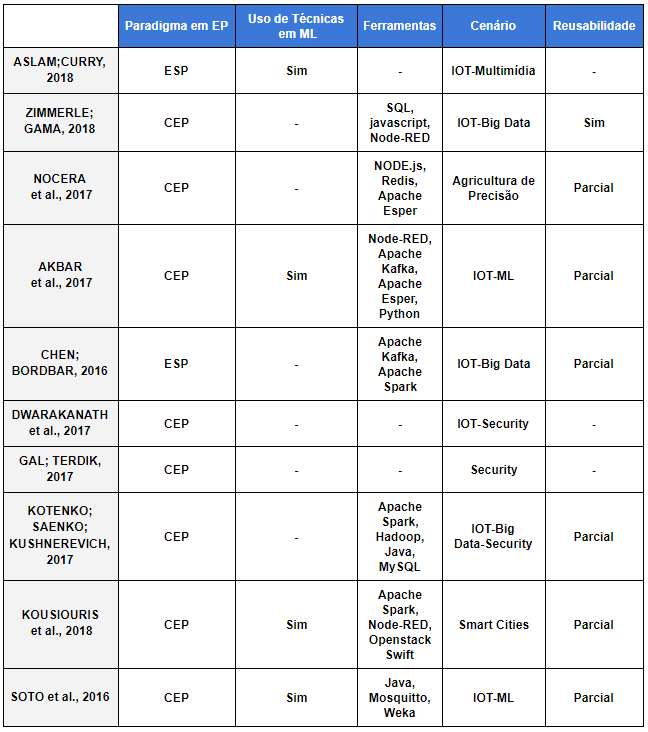
\includegraphics[width=1\textwidth]{imagens/comparacaoArtigos.png}
	\caption{Comparativo entre os artigos selecionados.}
	\label{fig:comparacaoArtigos}
\end{figure}


A partir da analise da figura \ref{fig:comparacaoArtigos} identificou-se que dentre os artigos selecionados durante o mapeamento apenas dois destes, \cite{art1aslam2018towards} e \cite{art5chen2016dress} trabalhavam com ESP, todos os demais trabalhos aplicam CEP de alguma forma em suas soluções. As técnicas de aprendizado de maquina também não foram usadas por muitos dos artigos selecionados, apenas quatro documentos fizeram uso desta tecnologia para solucionar os problemas abordados, os quais foram \cite{art1aslam2018towards}, \cite{art4akbar2017predictive}, \cite{art9kousiouris2018integrated} e \cite{art10soto2016ceml}. 

Um grande problema identificado dentre os Dez documentos selecionados foi a questão de reusabilidade, apenas \cite{art2zimmerle2018web} apresentou uma solução passível de reimplementação e reutilização completa, as demais não demonstraram detalhamento suficiente em suas propostas para que terceiros pudessem  fazer a reimplementação de suas abordagens e a remontagem das validações executados, demonstrando que as soluções não podem ser verificável e observável algo imprecisável em um documento cientifico. 

\section{Considerações do Capítulo}

Neste capítulo foi executado um mapeamento sistemático com o objetivo de  identificar o estado da arte em processamento de eventos para redes IoT. Como resultado deste mapeamento identificou-se alguns trabalhos de interesse onde foi elaborado um detalhamento de suas motivações e justificativas para a elaboração do mesmo, também foi detalhado a solução que cada um destes trabalhos propuseram e por ultimo foi apresentado os resultados que os autores obtiveram com o desenvolvimento destes trabalhos. Por fim foi demonstrada uma comparação entre as tecnologias empregadas em cada um destes trabalhos e apresentando criticas e desafios identificados durante esta revisão. 

%%%%%%%%%%%%%%%%%%%%%%%%%%%%%%%%%%%%%%%%%%%%%%%%%%%%%%%%%%%%%%%%%%%%%%%

\chapter{Considerações Finais}
\label{cap:Consideracoes_Finais}

O presente trabalho teve como objetivo fazer o levantamento dos trabalhos científicos elaborados sobre processamento de eventos aplicados a internet das coisas, onde para se atingir este objetivo foi executado um mapeamento sistemático o qual seguiu o algoritmo proposto por Petersen et al. (2008). Após a execução do mapeamento sistemático identificou-se dez trabalhos de interesse onde foi elaborada uma discussão comparando estes trabalhos entre si, onde identificou-se que a maioria dos autores destes trabalhos não se preocuparam com a reusabilidade de suas propostas oque dificulta a elaboração de novos trabalhos que façam uso ou mesmo que se baseiem nestas soluções.

%\section{Perspectiva de Investigação}

%\section{Trabalhos Futuros}

%%%%%%%%%%%%%%%%%%%%%%%%%%%%%%%%%%%%%%%%%%%%%%%%%%%%%%%%%%%%%%%%%%%%%%%
\bibliography{bibliografia}
\bibliographystyle{abnt}

\end{document}